\section{Quadro aggiornato degli esperimenti terminati}
\label{sec:completed-experiments-overview}
Questa sezione raccoglie i risultati finali disponibili negli archivi
esaminati il 26 ottobre 2026. Per i confronti sul corpus si includono
soltanto configurazioni terminate su tutti e dodici i dataset e su tutte
le ripetizioni previste. Una run con stato \texttt{completed} resta
inclusa anche se termina al limite iterativo senza convergere.
Gli stati \texttt{running}, \texttt{interrupted} e \texttt{not\_started}
non sono risultati finali e non sono sostituiti da zeri.

\subsection{Inventario delle esecuzioni e confronti ammessi}
Le versioni del prompt sono mantenute separate: cambiamenti di policy,
input o temperatura non consentono di interpretare le differenze fra
suite come effetto causale di un singolo fattore. Ogni voce dell'inventario
conta una run salvata, non una replica necessariamente indipendente;
eventuali riusi non costituiscono nuova evidenza sperimentale.
Nelle tabelle seguenti compaiono soltanto configurazioni concluse sui
dodici dataset e con metriche finali disponibili per entrambi i livelli.
Le configurazioni parziali non compaiono neppure nei conteggi riportati
in questo capitolo e non restringono la coorte delle medie.
\begin{table}[htbp]
\centering\small
\caption{Configurazioni incluse nei risultati: ogni configurazione comprende dodici run finali sui dodici dataset. Il numero di run include esclusivamente le configurazioni riportate, senza esecuzioni parziali.}\label{tab:completed-suite-inventory}
\begin{tabular}{llrl}
\toprule
Suite (data e ora) & Policy & Run incluse & Configurazioni complete \\
\midrule
20261023\_015718 & v63 & 72 & P4, P0, P1, T0, T4, T6 \\
20261023\_163929 & v72 & 12 & P4 \\
20261024\_005011 & v83 & 48 & P4, P0, P1, T0 \\
20261024\_211627 & v103 & 48 & P4, P0, P1, T0 \\
20261025\_170859 & v111 & 36 & P4, P0, P1 \\
\bottomrule
\end{tabular}
\end{table}
P0 e P1 indicano zero-shot e one-shot; P4 indica il riferimento
few-shot configurato nella relativa suite. T0, T4 e T6 identificano le
temperature 0,0, 0,4 e 0,6 del piano storico. Le impostazioni effettive
del riferimento sono riportate nella tabella successiva: non si assume
che siano identiche al piano corrente a temperatura 0,2.
Le suite senza metriche finali complete e verificate non vengono
riportate come risultati quantitativi.
\begin{table}[htbp]
\centering\small
\caption{Risultati definitivi delle configurazioni complete: esempi, temperatura, F1 macro e convergenza. Ogni riga comprende dodici dataset con output finali valutati; le suite sono confrontate separatamente.}\label{tab:completed-all-cohorts}
\begin{tabular}{lrrrrrr}
\toprule
Policy & Config. & Esempi & T & F1 HLG & F1 LLG & Convergenti \\
\midrule
v63 & P4 & 4 & 0,2 & 0,5445 & 0,5292 & 8/12 \\
v63 & P0 & 0 & 0,2 & 0,5334 & 0,5079 & 8/12 \\
v63 & P1 & 1 & 0,2 & 0,5473 & 0,5311 & 10/12 \\
v63 & T0 & 4 & 0,0 & 0,5266 & 0,5082 & 6/12 \\
v63 & T4 & 4 & 0,4 & 0,5376 & 0,5198 & 8/12 \\
v63 & T6 & 4 & 0,6 & 0,5387 & 0,5203 & 8/12 \\
v72 & P4 & 4 & 0,3 & 0,5185 & 0,5383 & 11/12 \\
v83 & P4 & 4 & 0,3 & 0,5321 & 0,5267 & 11/12 \\
v83 & P0 & 0 & 0,3 & 0,5304 & 0,5057 & 11/12 \\
v83 & P1 & 1 & 0,3 & 0,5376 & 0,5266 & 12/12 \\
v83 & T0 & 4 & 0,0 & 0,5410 & 0,5092 & 7/12 \\
v103 & P4 & 4 & 0,3 & 0,5372 & 0,5153 & 10/12 \\
v103 & P0 & 0 & 0,3 & 0,5418 & 0,5558 & 11/12 \\
v103 & P1 & 1 & 0,3 & 0,5428 & 0,5083 & 12/12 \\
v103 & T0 & 4 & 0,0 & 0,5373 & 0,5321 & 6/12 \\
v111 & P4 & 4 & 0,2 & 0,5207 & 0,5111 & 10/12 \\
v111 & P0 & 0 & 0,2 & 0,5422 & 0,5455 & 10/12 \\
v111 & P1 & 1 & 0,2 & 0,5271 & 0,5407 & 11/12 \\
\bottomrule
\end{tabular}
\end{table}
Le metriche provengono dagli export finali del notebook 04,
associati alla rispettiva suite; gli hash e i percorsi sono registrati
negli artefatti di questa analisi. Non si aggregano esportazioni ripetute
delle stesse run. I risultati storici v103 gi\`a discussi nelle sezioni
successive restano riferiti al loro snapshot originale; la tabella
qui sopra include anche T0, completata successivamente a quello snapshot.

\subsection{Risultati della suite v111 a temperatura 0,2}
La suite \path{ofat_fixed_thresholds_20261025_170859} usa gli input
schematici v111 e la soglia 0,68. P0, P1 e P4 hanno ciascuna dodici
run finali e condividono le stesse baseline congelate. Queste sono le
sole configurazioni della suite incluse nei risultati definitivi.
Le configurazioni di temperatura non ancora complete sono escluse
interamente, senza riportarne medie o conteggi parziali.
Le metriche vengono ricalcolate come medie aritmetiche delle righe
finali esportate, selezionando esplicitamente i dodici dataset comuni
a P0, P1 e P4. Si applica lo stesso filtro della sezione del notebook 04
dedicata alle configurazioni concluse su tutti i dodici dataset:
le configurazioni parziali non determinano l'intersezione del corpus.
Il matching usa
\texttt{bert-base-uncased}, le descrizioni dei goal e il preprocessing
NLTK; non applica la soglia MPNet 0,68 alla valutazione esterna.
La baseline \`e appaiata tramite dataset e identificativo della baseline.
\begin{table}[htbp]
\centering\small
\caption{Suite v111: Precision, Recall e F1 macro sui dodici dataset, con differenza assoluta di F1 dalla baseline appaiata. Una ripetizione per configurazione.}\label{tab:v111-final-macro}
\begin{tabular}{lrrrrrr}
\toprule
Metodo & Livello & Dataset & Precision & Recall & F1 & $\Delta$F1 \\
\midrule
Top-down & HLG & 12 & 0,5794 & 0,5725 & 0,5297 & +0,0000 \\
Top-down & LLG & 12 & 0,6866 & 0,4675 & 0,5083 & +0,0000 \\
P0 & HLG & 12 & 0,6017 & 0,5620 & 0,5422 & +0,0125 \\
P0 & LLG & 12 & 0,6863 & 0,5065 & 0,5455 & +0,0371 \\
P1 & HLG & 12 & 0,5958 & 0,5456 & 0,5271 & -0,0026 \\
P1 & LLG & 12 & 0,6726 & 0,5190 & 0,5407 & +0,0324 \\
P4 & HLG & 12 & 0,5596 & 0,5756 & 0,5207 & -0,0090 \\
P4 & LLG & 12 & 0,6710 & 0,4946 & 0,5111 & +0,0027 \\
\bottomrule
\end{tabular}
\end{table}
\begin{figure}[htbp]
\centering
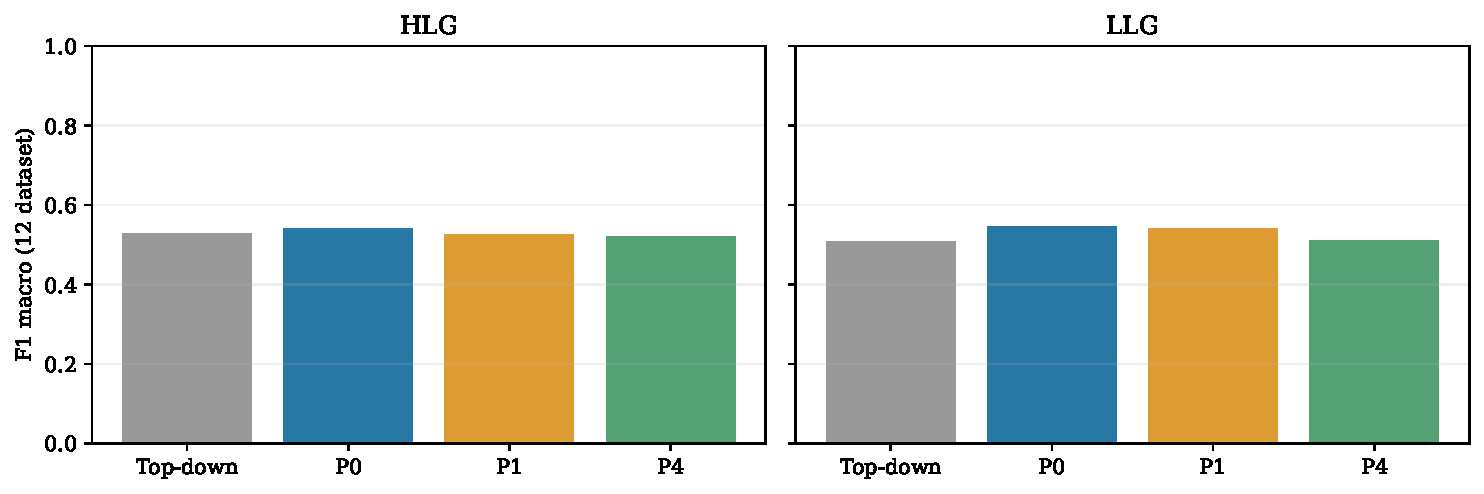
\includegraphics[width=\textwidth]{output/evaluation/completed_experiments_20261026/v111_macro_f1.pdf}
\caption{F1 macro della suite v111 e delle baseline. La scala comune 0--1 evita di amplificare visivamente differenze piccole.}\label{fig:v111-macro}
\end{figure}
P0 ottiene F1 HLG 0,5422 e
F1 LLG 0,5455, i valori maggiori
fra le tre configurazioni di questa suite. P4 ottiene invece F1 HLG
0,5207, sotto la baseline
0,5297, e F1 LLG
0,5111, poco sopra la baseline
0,5083. L'aggiunta di esempi non produce
quindi un miglioramento monotono. Le differenze sono descrittive:
una sola generazione per coppia dataset--configurazione non permette
di stimare stabilit\`a o significativit\`a dell'ordinamento.
\begin{table}[htbp]
\centering\small
\caption{Suite v111: differenze di F1 per dataset rispetto al proprio top-down. H e L indicano HLG e LLG.}\label{tab:v111-all-dataset-deltas}
\begin{tabular}{lrrrrrr}
\toprule
Dataset & P0 H & P0 L & P1 H & P1 L & P4 H & P4 L \\
\midrule
AUU & +0,0628 & -0,0089 & +0,1584 & +0,0219 & -0,0193 & +0,0309 \\
Calculator & +0,0000 & +0,0000 & +0,0000 & +0,0000 & +0,0000 & +0,0000 \\
Ethical Purchasing & +0,0000 & +0,0000 & +0,0000 & +0,0000 & +0,0000 & +0,0000 \\
Event Organization & -0,0069 & +0,2137 & -0,1032 & +0,2499 & -0,0263 & +0,0723 \\
Fitness Tracker & +0,0355 & +0,0192 & -0,1511 & +0,0189 & +0,0095 & -0,0199 \\
Genome Nexus & +0,0000 & +0,0000 & +0,0000 & +0,0000 & +0,0000 & +0,0000 \\
Gestao Hospital & +0,0000 & +0,0000 & +0,0000 & +0,0000 & +0,0000 & +0,0000 \\
La Reine Marlene & -0,0004 & +0,1075 & +0,0018 & +0,1133 & +0,0002 & +0,0276 \\
London Ambulance & -0,0055 & -0,0268 & -0,0028 & -0,1261 & +0,0116 & -0,1699 \\
Planning Poker & +0,0627 & +0,0298 & -0,0255 & -0,0284 & -0,0296 & -0,0856 \\
Recycling & +0,0423 & -0,0786 & +0,1071 & +0,0207 & -0,0942 & +0,0150 \\
SIA 25--26 & -0,0404 & +0,1898 & -0,0158 & +0,1181 & +0,0402 & +0,1624 \\
\bottomrule
\end{tabular}
\end{table}
\begin{figure}[htbp]
\centering
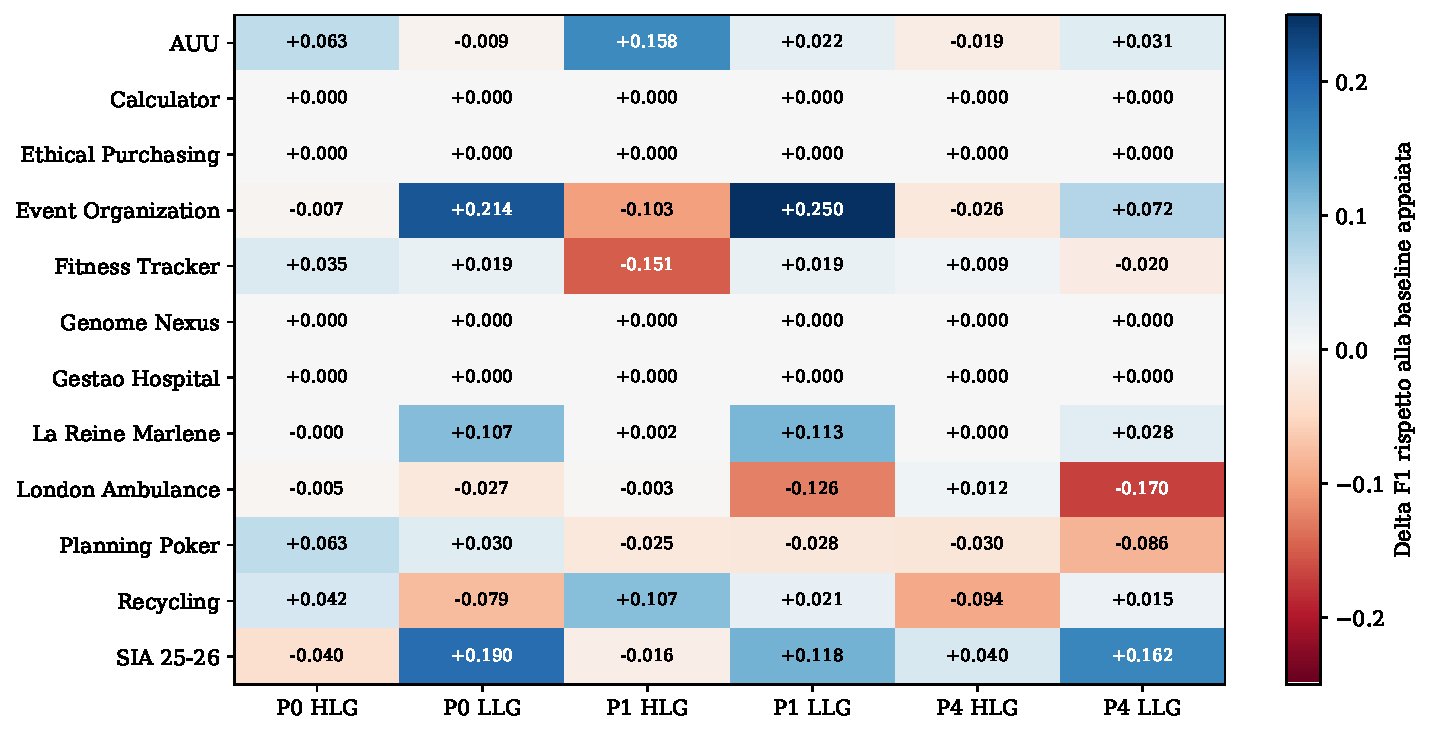
\includegraphics[width=\textwidth]{output/evaluation/completed_experiments_20261026/v111_dataset_deltas.pdf}
\caption{Variazioni di F1 per dataset nella suite v111. Blu indica aumento e rosso diminuzione rispetto alla stessa baseline; ogni cella conserva il valore numerico.}\label{fig:v111-deltas}
\end{figure}
I risultati non si muovono sempre insieme ai due livelli.
Nel riferimento P4, SIA 25--26 migliora soprattutto negli LLG
($\Delta$F1 = +0,1624), mentre London Ambulance peggiora negli LLG
($\Delta$F1 = -0,1699) pur migliorando leggermente negli HLG.
Calculator, Ethical Purchasing, Genome Nexus e Gestao Hospital
mantengono in P4 gli stessi punteggi della baseline. Una media vicina
alla baseline pu\`o quindi nascondere miglioramenti e peggioramenti
consistenti su singoli progetti. Una maggiore specificit\`a del testo
non coincide automaticamente con maggiore copertura o correttezza.

\subsection{Esempi di goal finali e interpretazione delle trasformazioni}
Gli estratti seguenti provengono dagli output finali \texttt{reference}
della suite v111, non dalle dimostrazioni fittizie del prompt.
La selezione comprende un miglioramento marcato, un peggioramento,
un effetto diverso tra livelli e un caso invariato; non rappresenta
un campionamento casuale n\'e una verifica manuale esaustiva dei requisiti.
\paragraph{SIA 25--26.}
Attore: Organization Office Staff. Padre iniziale: \emph{Ensure Efficient and Transparent Report Processing}.
\begin{quote}\small
\textbf{Ensure Efficient and Transparent Preliminary Review of Reports}\\
Organization Office Staff performs a preliminary review of citizen reports, marking them as accepted or rejected. A written justification is mandatory for rejections; other status changes (e.g., Pending Approval to In Progress) do not require explicit justification. The Organization Office is responsible for the preliminary review and rejection justification only.
\end{quote}
La formulazione finale restringe la responsabilit\`a dell'ufficio alla verifica preliminare e rende esplicita la motivazione del rifiuto, invece di attribuirgli l'intero processo fino alla risoluzione. Questa trasformazione illustra una correzione dei confini di responsabilit\`a; l'aumento di F1 degli LLG riguarda l'intero dataset e non pu\`o essere attribuito causalmente a questo solo padre.
La descrizione iniziale era: \emph{Provide a structured workflow for reports to move through approval, assignment, and resolution stages with clear state transitions and accountability.}.
\paragraph{London Ambulance.}
Attore: Ambulance Driver. Padre iniziale: \emph{Ensure timely ambulance response}.
\begin{quote}\small
\textbf{Ensure timely ambulance response}\\
Allocate an available ambulance for every emergency call that can reach the scene within 11 minutes, by following standard routes and communicating departure and destination information to support real-time dispatch.
\end{quote}
Il dataset presenta un piccolo aumento di F1 HLG ma una diminuzione marcata di F1 LLG. L'esempio mostra il contenuto di un padre finale; il peggioramento quantitativo della decomposizione non dimostra, da solo, che ogni sua frase sia errata. Cambiamenti di granularit\`a, cardinalit\`a e corrispondenza con il riferimento possono contribuire al punteggio: stabilire il peso di ciascun fattore richiede un'analisi delle singole corrispondenze.
La descrizione iniziale era: \emph{Minimize response time to ensure every emergency call is reached within 11 minutes.}.
\paragraph{Event Organization.}
Attore: Service Provider. Padre iniziale: \emph{Offer and Market Services to Event Clients}.
\begin{quote}\small
\textbf{Offer and Manage Event-Related Services}\\
Allow service providers to showcase their services, receive and manage appointment requests, prepare and upload quotations, and handle payments associated with confirmed appointments.
\end{quote}
Il padre finale esplicita gestione delle richieste di appuntamento, preventivi e pagamenti associati agli appuntamenti confermati. Il risultato complessivo aumenta F1 LLG (+0,0723), ma riduce F1 HLG (-0,0263): una descrizione pi\`u dettagliata e una decomposizione pi\`u vicina al riferimento possono coesistere con una minore corrispondenza al livello superiore.
La descrizione iniziale era: \emph{Allow service providers to showcase their services, receive appointment requests, and manage payments in a transparent and efficient manner.}.
\paragraph{Calculator.}
Attore: User. Padre iniziale: \emph{Enable quick and accurate basic arithmetic operations}.
\begin{quote}\small
\textbf{Enable quick and accurate basic arithmetic operations}\\
Provide users with a reliable and intuitive interface to perform fundamental calculations such as addition, subtraction, multiplication, and division.
\end{quote}
Il padre rimane identico alla baseline e i punteggi HLG e LLG non cambiano. La revisione pu\`o quindi confermare un risultato gi\`a presente; assenza di modifica e assenza di miglioramento non equivalgono a un fallimento tecnico.
La descrizione iniziale era: \emph{Provide users with a reliable and intuitive interface to perform fundamental calculations such as addition, subtraction, multiplication, and division.}.
\subsection{Esperimento esplorativo sulla soglia cosine}
\label{sec:completed-threshold-results}
L'esperimento di soglia \`e distinto dalle run iterative precedenti:
ricostruisce HLG$'$ dalle baseline dei dodici dataset e calcola i
punteggi delle coppie, senza rieseguire l'intera pipeline per ogni
valore ipotizzato. Sono disponibili 60 ricostruzioni rispetto a 61
padri iniziali: un padre privo di figli non viene ricostruito.
Le 394 coppie comprendono 60 confronti col padre e 334 con altri
HLG del progetto; fra questi ultimi, 112 riguardano lo stesso attore.
La media cosine HLG$'$--padre \`e 0,692983 e la media delle medie
per dataset \`e 0,697144. Sono statistiche di similarit\`a testuale,
non misure di accuratezza delle decisioni degli evaluator.
Le motivazioni, la copertura per dataset e tutti i punteggi sono
documentati nella Sezione~\ref{sec:cosine-tuning-all-datasets} e
nell'appendice dei valori completi.
\begin{table}[htbp]
\centering\small
\caption{Analisi di sensibilit\`a sulle stesse coppie: numero di padri sopra soglia e di altri HLG dello stesso attore sopra soglia. Non sono dieci run iterative n'e conteggi di veri duplicati.}\label{tab:completed-threshold-grid}
\begin{tabular}{lrr}
\toprule
Soglia & Padri sopra soglia / 60 & Altri HLG sopra soglia / 112 \\
\midrule
0,5 & 56 & 29 \\
0,55 & 54 & 20 \\
0,6 & 46 & 10 \\
0,65 & 39 & 6 \\
0,68 & 34 & 5 \\
0,7 & 29 & 5 \\
0,75 & 21 & 2 \\
0,8 & 13 & 0 \\
0,85 & 2 & 0 \\
0,9 & 0 & 0 \\
\bottomrule
\end{tabular}
\end{table}
\begin{figure}[htbp]
\centering
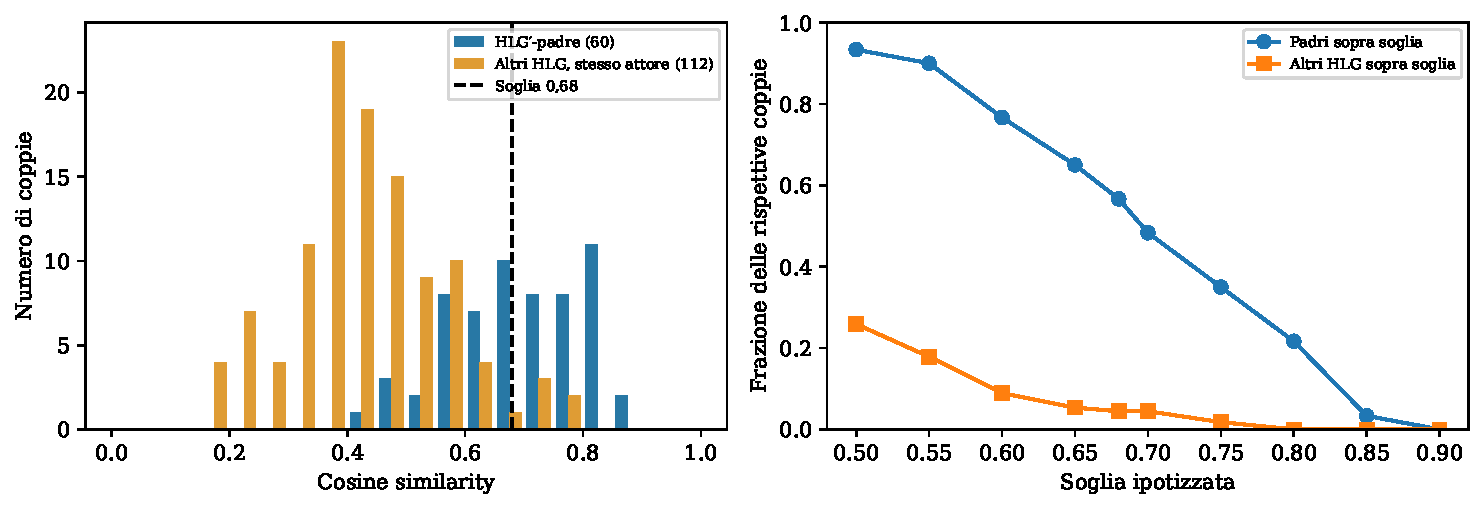
\includegraphics[width=\textwidth]{output/evaluation/completed_experiments_20261026/threshold_analysis.pdf}
\caption{Distribuzione dei punteggi e sensibilit\`a dello screening alla soglia. Le frazioni a destra hanno denominatori diversi (60 e 112); non rappresentano Recall o tasso di falsi positivi.}\label{fig:completed-threshold-analysis}
\end{figure}
Una soglia pi\`u bassa aumenta sia le relazioni considerate equivalenti
sia i candidati duplicati da verificare; una soglia pi\`u alta restringe
entrambi gli insiemi. Il valore operativo 0,68 viene quindi descritto
come scelta esplorativa sulla distribuzione osservata. Senza annotazioni
indipendenti delle coppie non \`e possibile affermare che massimizzi
Precision, Recall o qualit\`a della gerarchia finale.
La tabella rende osservabile la sensibilit\`a, ma non dimostra
che uno dei valori sia ottimale.
\paragraph{Coppia reale: AUU.}
HLG$'$: \emph{Validate fiscal codes for children against national databases to ensure uniqueness and avoid conflicts.}. HLG confrontato: \emph{Enable real-time fiscal code validation and conflict detection}; descrizione: \emph{Prevent duplicate or conflicting applications by validating child fiscal codes in real time and blocking submissions when a child is already associated with another active application.}. Cosine = 0,6758; confronto col padre. Il punteggio non raggiunge la soglia 0,68; tale esito numerico non sostituisce il controllo documentale.
\paragraph{Coppia reale: SIA 25--26.}
HLG$'$: \emph{Provide public access to aggregated statistics on report trends and categories.}. HLG confrontato: \emph{Enable Public Access to Urban Issue Statistics}; descrizione: \emph{Allow non-registered users to view public statistics on report trends and categories to promote awareness and data-driven urban planning.}. Cosine = 0,6818; confronto col padre. Il punteggio supera la soglia 0,68; tale esito numerico non sostituisce il controllo documentale.
\paragraph{Coppia reale: Fitness Tracker.}
HLG$'$: \emph{Support user-defined fitness goals with milestone tracking and real-time feedback}. HLG confrontato: \emph{Enable users to track and analyze their physical activities}; descrizione: \emph{Provide a comprehensive platform for users to log, visualize, and interpret their workout data to understand performance trends.}. Cosine = 0,6672; confronto con un altro HLG. Il punteggio non raggiunge la soglia 0,68; tale esito numerico non sostituisce il controllo documentale.
\subsection{Sintesi dei risultati ottenuti}
Le esecuzioni concluse mostrano che la revisione pu\`o modificare
copertura, responsabilit\`a e granularit\`a dei goal, oppure lasciare
intatta la baseline. Nella suite v111, P0 ottiene la media maggiore
fra le configurazioni complete, mentre P4 produce guadagni e perdite
molto diversi tra dataset. Gli esempi nel prompt sono quindi una guida
decisionale da valutare, non una garanzia di miglioramento.
L'analisi cosine descrive quali coppie vengono sottoposte a tale giudizio;
non valida autonomamente la correttezza delle azioni. Le conclusioni
restano circoscritte alle run terminate, a una ripetizione e al matching
testuale adottato. Le analisi storiche che seguono conservano il loro
perimetro e non vengono reinterpretate come risultati della v111.
